
% Here comes a beautiful introduction. %Promise!

To begin with, we shall clarify the intended ambiguity of this work's title. Before approaching the question behind this thesis in the context of Representational Learning (RL), we would like to present it from a philosophical point of view of AI safety and potential.
One could argue, that we live in times of the fastest advances in science and technology in the history of humanity, therefore making us the \textit{Knowledge Generation}. While we continuously keep researching and accumulating knowledge, we have historically not been willing to share our knowledge with any other species in this Universe. All scientific milestones are from us, for us. 

The rise of AI marked a turning point of this tradition. For the first time we invest in sharing our knowledge and with systems which can act on superhuman dimension. While machine learning models might not be considered a species, they have learned to drive our cars and in fact beaten human intelligence in the game GO \cite{silver_mastering_2017}. This is not only seen as progress but also as danger. The world's richest man, Elon Musk, both build his fortune on AI and respects it as humanity's biggest risk. 

\begin{figure}[H]
    \centering
    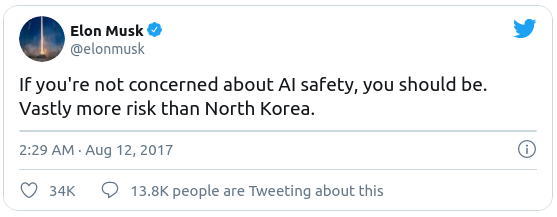
\includegraphics[height=.21\textwidth, keepaspectratio]{data/images/ElonMusk.png}
    \caption{Elon Musk in a tweet on AI. Source \cite{noauthor_elon_nodate}}
    \label{fig1:Elon}
\end{figure}


% \begin{figure}[H]
%     \centering
%     
\includepdf[pages=-,pagecommand={},width=\textwidth]{data/images/Elon75a4.pdf}
%     \caption{Elon Musk Tweet on AI. Source \cite{twitter}}
%     \label{fig1:Elon}
% \end{figure}


Closing the circle to the ambiguity of the title and relating to the popular concern, that AI might reach a point where it does not need humans anymore to keep evolving, we ask the crucial question: Can AI generate knowledge? 


\subsection{Motivation}

A key area of AI is RL, where the model learns to identify and disentangle characteristics and features of the data. Understanding the semantics of the data is specifically important for unsupervised learning of generative models. 
% computer vision
The task of generating data has been widely explored for images. Computer vision has reached a point where a simple image can be semantically segmented, where objects can be detected and classified and even relations between entities inferred \cite{kipf_contrastive_2020}.

% molecular graphs
Advances in the parallel field of graph generation have received less attention, yet showed promising results. Data stored as a graph has a high density of information and rich semantics, which makes it attractive for variational inference. The recent success of Simonovsky et al. \cite{simonovsky_graphvae_2018} on the generation and completion of molecules represented in graph structure, initially inspired our research. Next to molecules, graphs can be used to store knowledge. While real world Knowledge Graphs (KG) have a far higher complexity than molecule graphs, the proposed generative model, Variational Auto-Encoder (VAE) also has proven its capacity to learn from huge datasets with high variance. Inspired by Simonovsky work and motivated by the vision of generating knowledge, we explore the possibilities and limitation of KG generation with VAEs.



\subsection{Expected Contribution}

The main contributions of this thesis are threefold. The main objective is to proof the hypothesis that a graph VAE can capture, disentangle and reproduce the underlying semantics of a real world KG, secondly. Further we contribute with a novel implementation of a graph matching algorithm and a validation method for generated triples. 

In Simonovsky \cite{simonovsky_graphvae_2018} work, small subgraphs with multiple edges are used to represent molecule graphs. In contrast we proof the hypothesis by generating the smallest possible graph of two nodes, also representable as single triple. The VAE is tested and evaluated in several experiments, including link prediction, latent space interpolation and accuracy of generating valid triples.
% Proof of concept KGVAE


% draw parallels to molecules and explore the differences
We compare our results to related KGs methods and investigate the impact of different hyperparameter. The main focus is be on the influence of the graph matching loss function, the encoding through graph convolutions and stochastic inference. Further, we aim to reproduce the success of molecule generation and point therefore continuously the similarities and differences to our work out.

% Implementation of graph matching in batches
On a lower level, we hope to contribute with our implementation of Cho's \textit{et al.} max-pooling graph matching algorithm for tensor batches. While the algorithm has been cited and implemented numerous times, a working implementation, compatible with deep learning libraries, has to the best of our knowledge not yet been published.  

% Method for syntax cohearence of generated triples from real world KG
Lastly we introduce a high-level method for evaluating the validity of generated data, which compares the type constrain of the generated triple's predicate with its entity types and reports accuracy. This is made possible by expanding the existing dataset FB15K-237 with entity types from its original KG Freebase. While this scoring method is error prone, it does give an insight into the level representational potential of the model and the syntax coherence of the generated triples. Future work can use this evaluation method to track progress and compare to the baseline. 


% This thesis is aimed to be a proof of concept, providing insight into the capability of the VAE on generating KG triples and to indicate if further research in this direction would be meaningful.

\subsection{Research Question}

\begin{center}
    \texttt{How successful is a graph VAE in representation learning of real world KG compared to molecule graph data and what is the impact of each major hyperparameter?}
    \label{sec1:requestion}
\end{center}

% \emojismile

% Without further ado -
